En esta secci\'on, presentaremos los resultados obtenidos en los experimentos
utilizando lo definido en la secci\'on de desarrollo.

\subsection{Nodos distinguidos}

En cada experimento se analizaron las dos fuentes de información y se definió
un criterio para distinguir un nodo de cada red. Este criterio consta en que
será distinguido el simbolo con mas probabilidad de ocurrir o equivalentemente
el simbolo que tenga menor información.

Para la fuente $S_2$ una de las hipotesis es que estos nodos "distinguidos" son
nodos especiales como routers, access points, etc. dado que estos participan
en la mayor parte de las comunicaciones con la red como con el exterior.
Por lo cual esto nos daría un método (no 100\% confiable debido a casos
atípicos) de determinar los router en una red.

Otra de las hipotesis que se presenta es que una red \textit{cableada} será
mas "compresible" que una \textit{wireless}. Para esto se mostraron el
cociente de la $\frac{H(S)}{H_{MAX}(S)}$ como se desarrollo en TODO: CITA
y se los comparo entre el mismo tipo de fuente de los distintos experimentos.

\subsection{Descripción de los Gráficos}

En cada experimentación se generaron tres tipos de resultados/graficos.

\begin{itemize}
	\item Un gráfico que muestra una representación tipo torta de la fuente, esto es, la probabilidad de ocurrencia de cada simbolo.
	\item Un gráfico tipo histograma que muestra para cada símbolo la información de este. Este grafico cuenta además con una barra
	horizontar que muestra donde se situa la Entropía de la fuente (en color naranja) y otra barra similar que muestra donde
	se situa la Entropía maxima que podria tener la fuente.
	\item Un gráfico con la topologia de los mensajes de la red. Donde los nodos son \textbf{MAC} address y las
	aristas representan un paquete de un nodo a otro
\end{itemize}

\subsection{Red hogareña}

\subsubsection{Fuente Unicast-Multicast}

\hspace*{-1.5cm}
 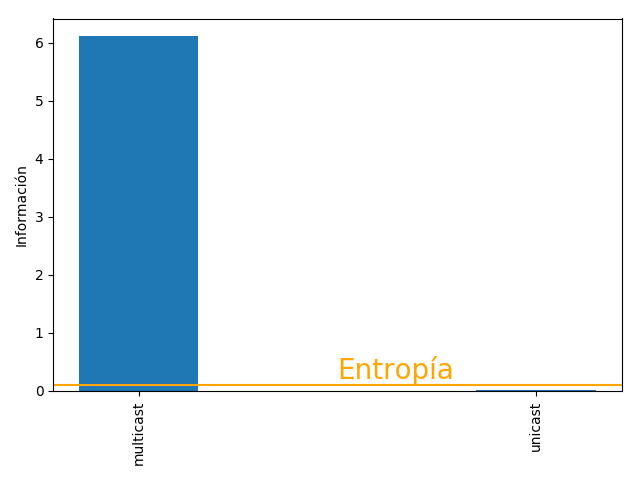
\includegraphics[scale=0.6]{../plots/mauro_s1_informacion.png}
 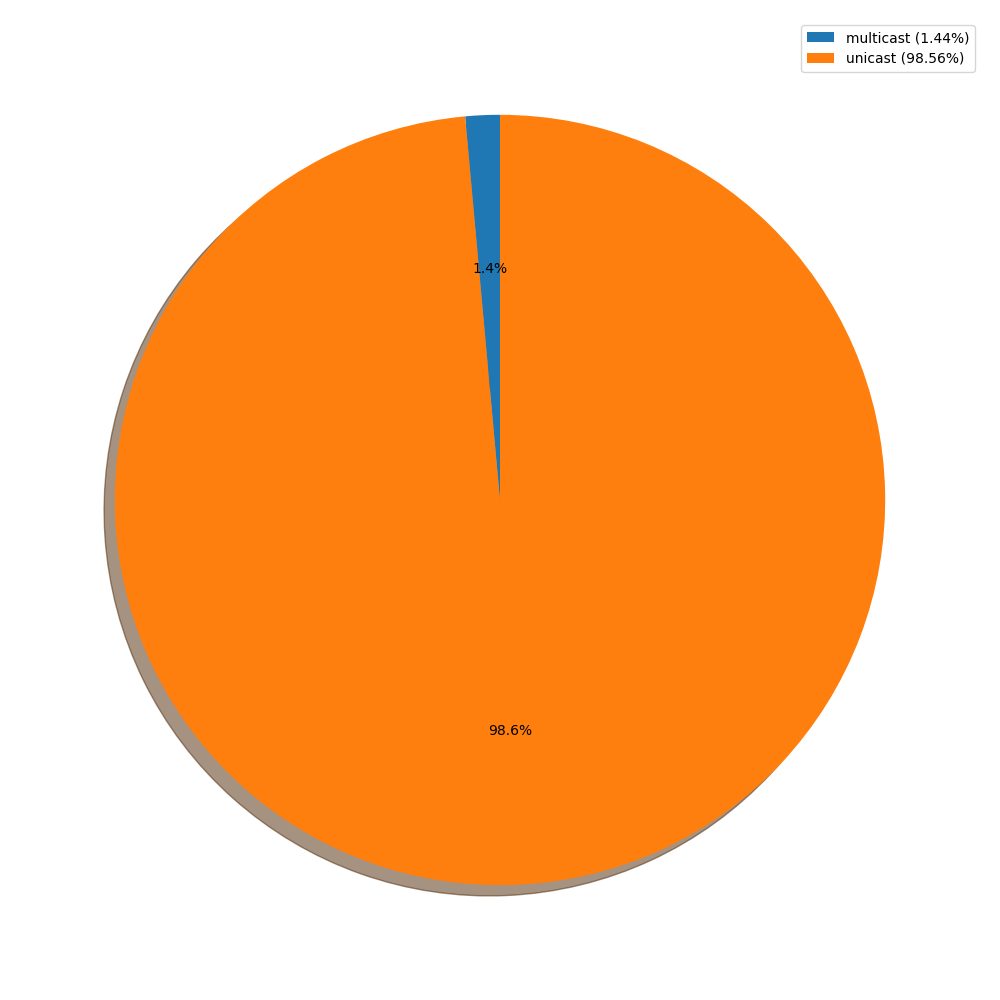
\includegraphics[scale=0.4]{../plots/mauro_s1_probabilidades.png}

Como podemos ver 
\subsubsection{Fuente ARP}

\hspace*{-1.5cm}
 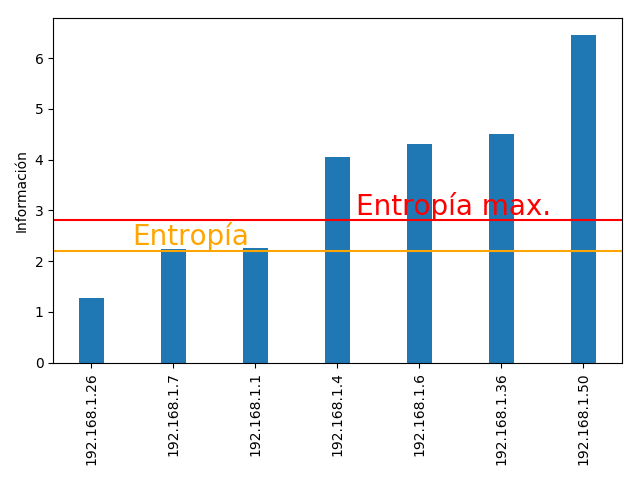
\includegraphics[scale=0.6]{../plots/mauro_s2_informacion.png}
 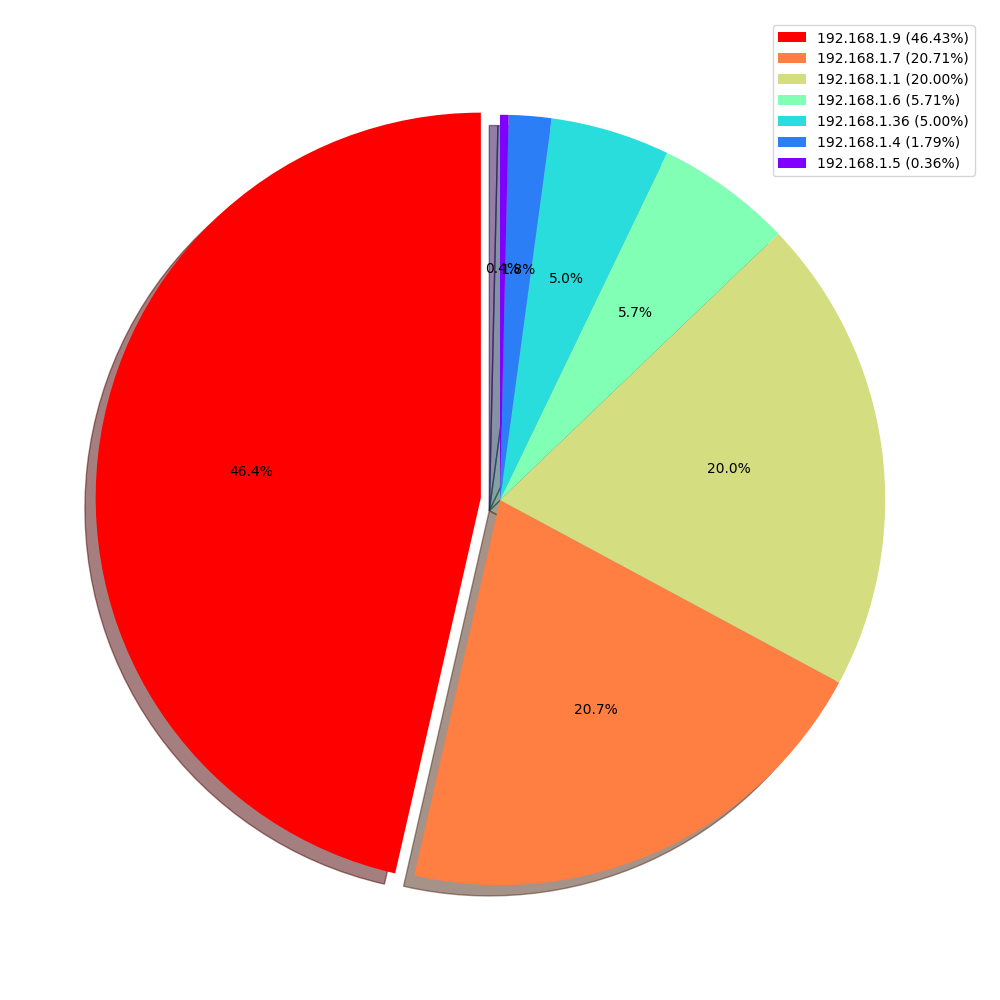
\includegraphics[scale=0.4]{../plots/mauro_s2_probabilidades.png}

\subsubsection{Topolog\'ia de la Red}
\begin{center}
 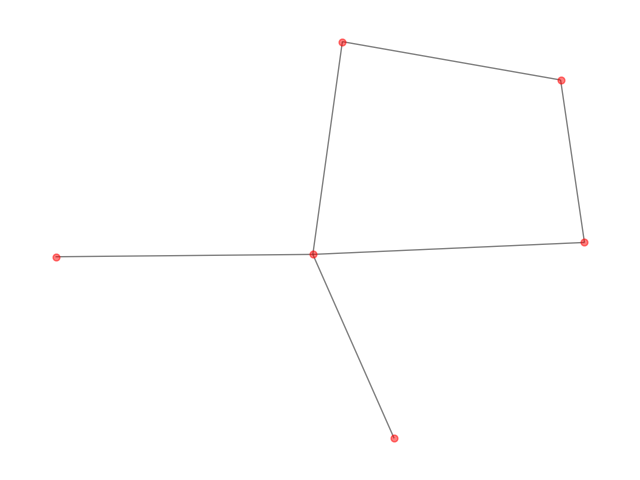
\includegraphics[scale=0.6]{../plots/mauro_s2_topologia.png}
\end{center}

\subsection{Experimento Chino}

\subsubsection{Fuente Unicast-Multicast}

\hspace*{-1.5cm}
 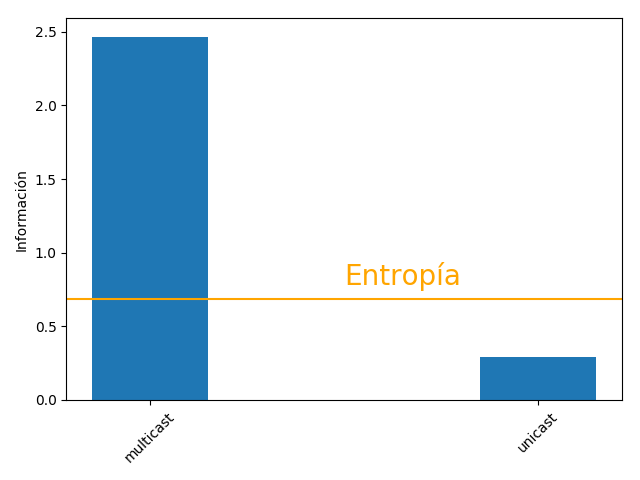
\includegraphics[scale=0.6]{../plots/trabajo_s1_informacion.png}
 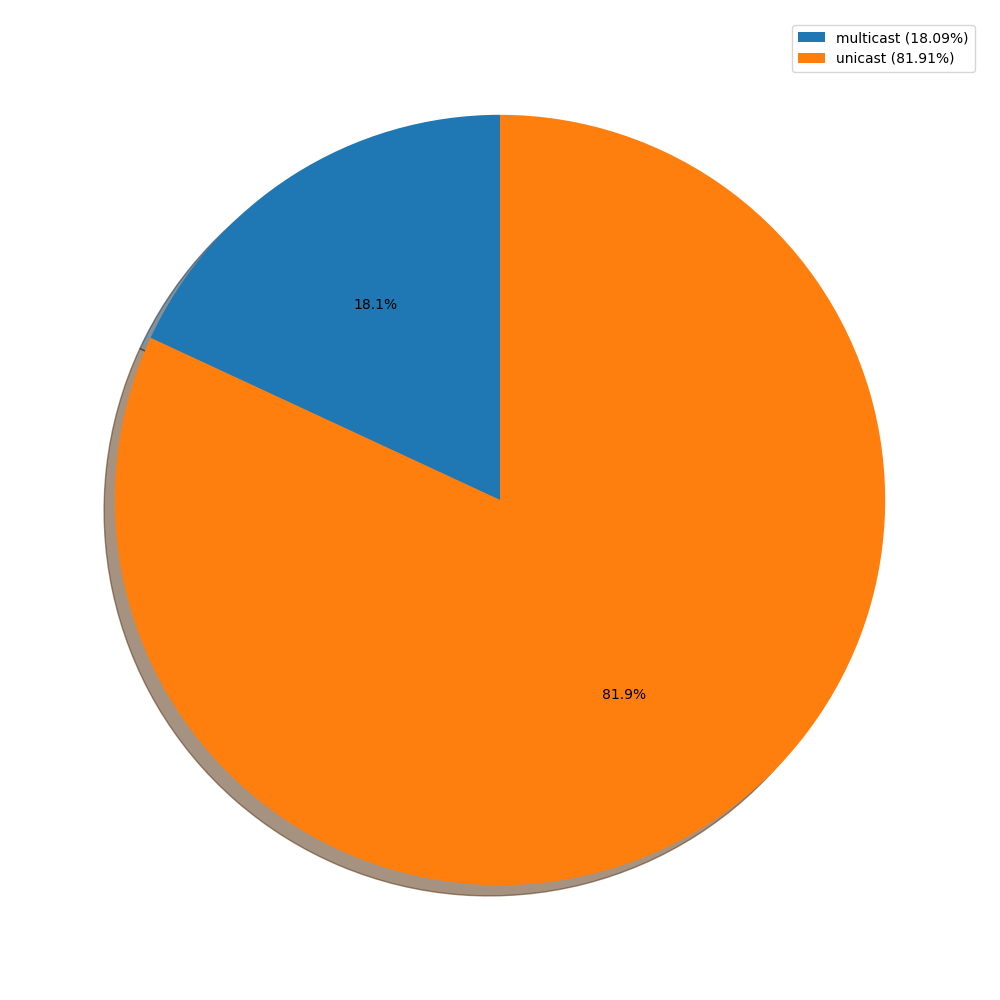
\includegraphics[scale=0.4]{../plots/trabajo_s1_probabilidades.png}

\subsubsection{Fuente ARP}

\hspace*{-1.5cm}
 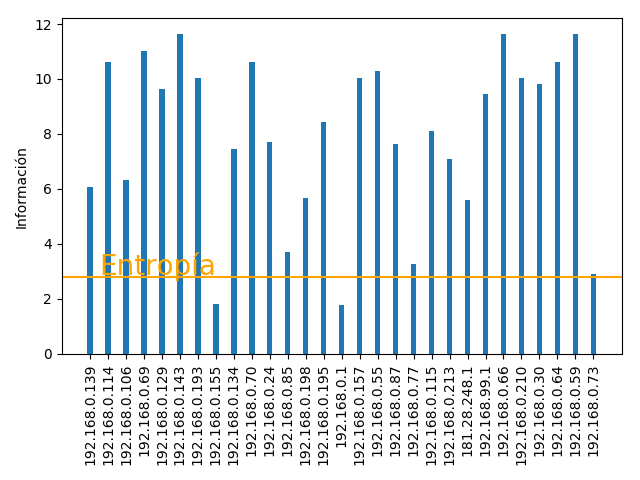
\includegraphics[scale=0.6]{../plots/trabajo_s2_informacion.png}
 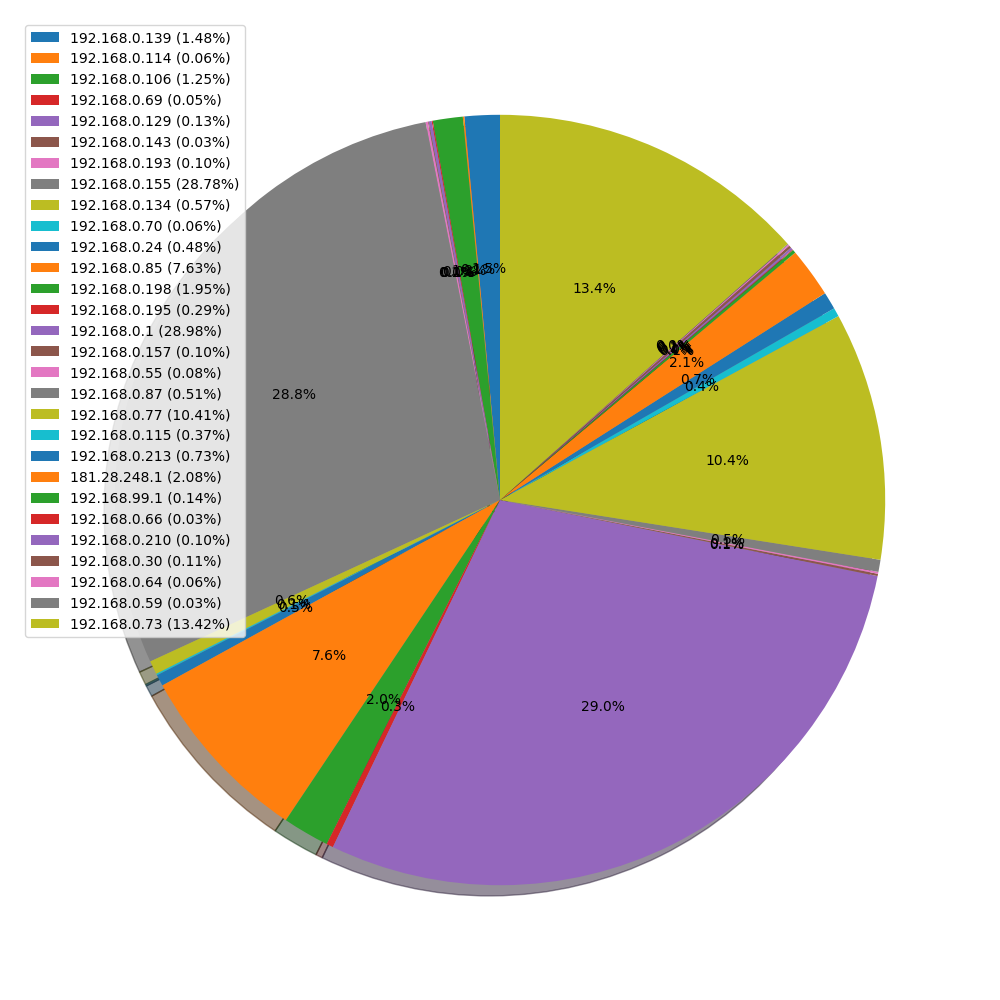
\includegraphics[scale=0.4]{../plots/trabajo_s2_probabilidades.png}


\subsubsection{Topolog\'ia de la Red}
\begin{center}
 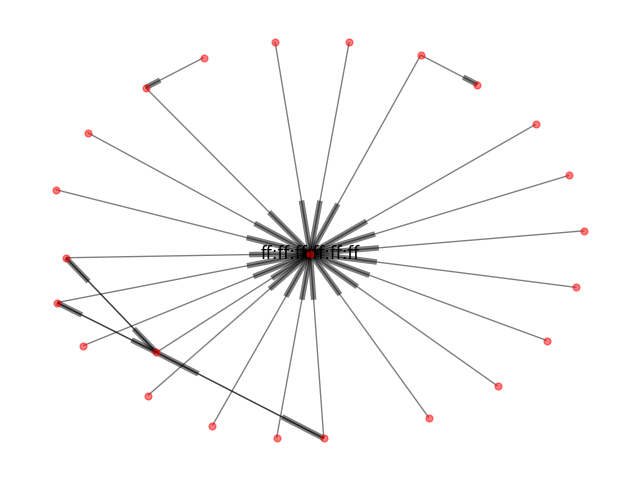
\includegraphics[scale=0.6]{../plots/trabajo_s2_topologia.png}
\end{center}

\subsection{Experimento Tavo}

Arreglar cosas